\documentclass[twoside,twocolumn]{article}

\usepackage{blindtext} % Package to generate dummy text throughout this template 
\usepackage{graphicx}
\usepackage[sc]{mathpazo} % Use the Palatino font
\usepackage[T1]{fontenc} % Use 8-bit encoding that has 256 glyphs
\linespread{1.05} % Line spacing - Palatino needs more space between lines
\usepackage{microtype} % Slightly tweak font spacing for aesthetics

\usepackage[english]{babel} % Language hyphenation and typographical rules

\usepackage[hmarginratio=1:1,top=32mm,columnsep=20pt]{geometry} % Document margins
\usepackage[hang, small,labelfont=bf,up,textfont=it,up]{caption} % Custom captions under/above floats in tables or figures
\usepackage{booktabs} % Horizontal rules in tables

\usepackage{lettrine} % The lettrine is the first enlarged letter at the beginning of the text

\usepackage{enumitem} % Customized lists
\setlist[itemize]{noitemsep} % Make itemize lists more compact

\usepackage{abstract} % Allows abstract customization
\renewcommand{\abstractnamefont}{\normalfont\bfseries} % Set the "Abstract" text to bold
\renewcommand{\abstracttextfont}{\normalfont\small\itshape} % Set the abstract itself to small italic text

\usepackage{titlesec} % Allows customization of titles
\renewcommand\thesection{\Roman{section}} % Roman numerals for the sections
\renewcommand\thesubsection{\roman{subsection}} % roman numerals for subsections
\titleformat{\section}[block]{\large\scshape\centering}{\thesection.}{1em}{} % Change the look of the section titles
\titleformat{\subsection}[block]{\large}{\thesubsection.}{1em}{} % Change the look of the section titles

\usepackage{fancyhdr} % Headers and footers
\pagestyle{fancy} % All pages have headers and footers
\fancyhead{} % Blank out the default header
\fancyfoot{} % Blank out the default footer
\fancyhead[C]{Herramientas de Gestion de Pruebas $\bullet$ Noviembre 2021 } % Custom header text
\fancyfoot[RO,LE]{\thepage} % Custom footer text

\usepackage{titling} % Customizing the title section

\usepackage{hyperref} % For hyperlinks in the PDF
% Keywords command
\providecommand{\keywords}[1]
{
  \small	
  \textbf{\textit{Keywords---}} #1
}

%----------------------------------------------------------------------------------------
%	TITLE SECTION
%----------------------------------------------------------------------------------------
\begin{document}
\begin{titlepage}
\begin{center}
\large{UNIVERSIDAD PRIVADA DE TACNA}\\
\vspace*{-0.025in}
\begin{figure}[htb]
\begin{center}
	
\includegraphics[width=5cm]{./imagenes/logo.jpg} 
\end{center}
\end{figure}
\vspace*{0.15in}
INGENIERIA DE SISTEMAS  \\

\vspace*{0.5in}
\begin{large}
\textbf{TITULO:}\\
\end{large}

\vspace*{0.1in}
\begin{Large}
TRABAJO ENCARGADO N° 01: HERRAMIENTAS DE GESTION DE PRUEBAS \\
\end{Large}

\vspace*{0.3in}
\begin{Large}
\textbf{CURSO:} \\
\end{Large}

\vspace*{0.1in}
\begin{large}
CALIDAD Y PRUEBAS DE SOFTWARE\\
\end{large}

\vspace*{0.3in}
\begin{Large}
\textbf{DOCENTE:} \\
\end{Large}

\vspace*{0.1in}
\begin{large}
 Patrick Cuadros Quiroga\\
\end{large}

\vspace*{0.2in}
\vspace*{0.1in}
\begin{large}
Integrantes: \\
\begin{flushleft}
Anahua Huayhua, Jenny Karen		\hfill	(2018062150) \\
Coloma Colquehuanca, Kiara Estefani		\hfill	(2018062218) \\
Cuadros Napa, Raul Marcelo         	\hfill	(2017057851) \\
Limache Durand, Rodrigo Jeral      	\hfill	(2017059278) \\
\end{flushleft}
\end{large}
\vspace*{0.8in}
Tacna - Peru\end{center}
\begin{center}
2021\end{center}
\end{titlepage}
\setlength{\droptitle}{-4\baselineskip} % Move the title up
\pretitle{\begin{center}\Huge\bfseries} % Article title formatting
\posttitle{\end{center}} % Article title closing formatting
\title{Herramientas de gestión de pruebas} % Article title
\author{Jenny Anahua, Kiara Coloma, Raul Cuadros y Rodrigo Limache}
\date{\today} % Leave empty to omit a date
\renewcommand{\maketitlehookd}{%
\begin{large}
\centering Resumen\\
\end{large}
\vspace{0.5cm}
\noindent En la presente articulo nos dedicamos a indagar sobre las peculiaridades de plataformas de Cloud Computing. Es el caso de Azure Devops, AWS Codepipeline, Google Code Build, Github Actions, etc , haciendo uso de versiones privadas de prueba en entornos educativos. Teniendo en cuenta sus características principales, se procede a realizar una comparación de las plataformas mencionadas, con la finalidad de elaborar una Tabla comparativa de los frameworks mencionados para presentar una serie de recomendaciones acerca de las características de las plataformas más seguras y adecuadas a la hora de decidir por una u otra. Con el fin de alcanzar el objetivo de este trabajo que resulta ser el de indagar y adquirir conocimientos teóricos sobre marcos de trabajo de plataformas de Cloud Computing
\begin{abstract}
\noindent In this article we are dedicated to investigating the peculiarities of Cloud Computing platforms. This is the case of Azure Devops, AWS Codepipeline, Google Code Build, Github Actions, etc., making use of private trial versions in educational environments. Taking into account their main characteristics, a comparison of the aforementioned platforms is carried out, in order to prepare a comparative table of the aforementioned frameworks to present a series of recommendations about the characteristics of the safest and most appropriate platforms at the time to decide for one or the other. In order to achieve the objective of this work, which turns out to be to investigate and acquire theoretical knowledge about Cloud Computing platform frameworks. 
\end{abstract}
\keywords{Test, Pruebas, Software, Calidad,Azure Devops,Google Code Build}
}
%----------------------------------------------------------------------------------------


% Print the title
\maketitle
%----------------------------------------------------------------------------------------
%	ARTICLE CONTENTS
%----------------------------------------------------------------------------------------
\section{Introduccion}

\lettrine[nindent=0em,lines=3]{L}as herramientas de gestión de pruebas son aquellas que se utilizan para gestionar la información relativa a los «casos de prueba», normalmente los funcionales, para planificar actividades de testing, para gestionar los informes resultantes después de pasar dichos test, etc.
Es fundamental para cualquier proyecto, salvo que sea muy pequeño, contar con alguna herramienta de gestión de pruebas. Hay herramientas que van por separado y otras que integran con herramientas complementarias, por ejemplo, con las de «bug tracking».

%------------------------------------------------
\section{Objetivos}

\begin{itemize}
\item Conocer sobre Herramientas de pruebas.
\end{itemize}
%------------------------------------------------
\section{Desarrollo}
\subsection{HERRAMIENTAS DE GESTIÓN DE PRUEBAS}
Las herramientas de gestión de pruebas ayudan a gestionar todo el ciclo de pruebas de un producto. Una herramienta de gestión de pruebas útil debería poder integrarse con otros marcos de automatización y Integración CI.\\
Las tareas de automatización de pruebas están cada vez más presentes en el mercado para automatizar las tareas de prueba. Existen una serie de herramientas de automatización, pero es poco probable que una sola herramienta pueda automatizar todas las tareas de prueba. La mayoría de las herramientas se centran en una tarea o grupo de tareas específicas, aunque algunas sólo tratan un aspecto de la tarea.
\begin{center}
	
\includegraphics[width=6.5cm]{./imagenes/testing.jpg} 
	\end{center}
\subsection{Algunas Herramientas de gestion de Pruebas}
\begin{itemize}
    \item XRAY\\
Radiografía es una de las herramientas de gestión de pruebas preferidas para pruebas manuales y automatizadas. Proporciona la estructura adecuada para organizar y clasificar conjuntos de pruebas y proporciona resultados de prueba eficientes en menos tiempo\\
\begin{center}
	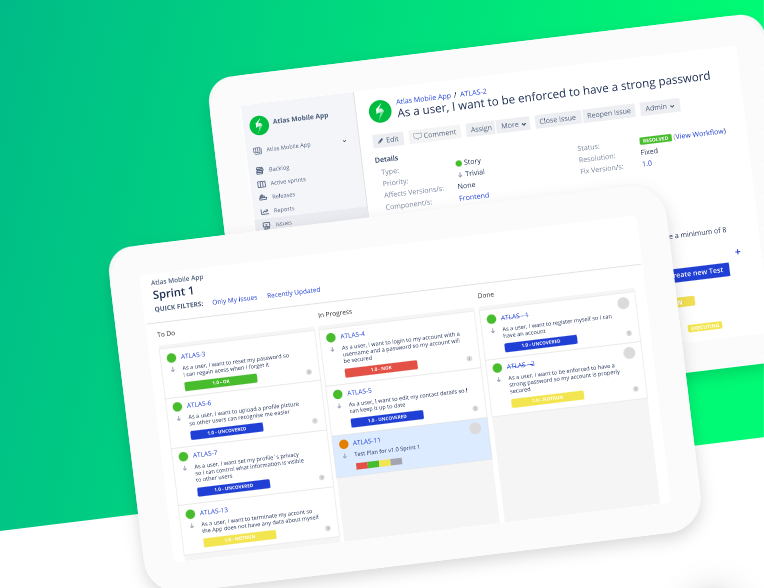
\includegraphics[width=6.5cm]{./imagenes/xray.png} 
	\end{center}
    \item TESTRAIL\\
TestRail es una herramienta de gestión de casos de prueba basada en la web que se puede configurar y utilizar fácilmente con la nube o la configuración local. Es altamente escalable y personalizable. Puede ver información en tiempo real sobre el progreso de las pruebas a través de paneles interactivos, métricas, informes de actividad, etc. Los casos de prueba automáticos y manuales se pueden administrar y documentar fácilmente mediante capturas de pantalla, comparación de resultados esperados versus reales.\\
\begin{center}
	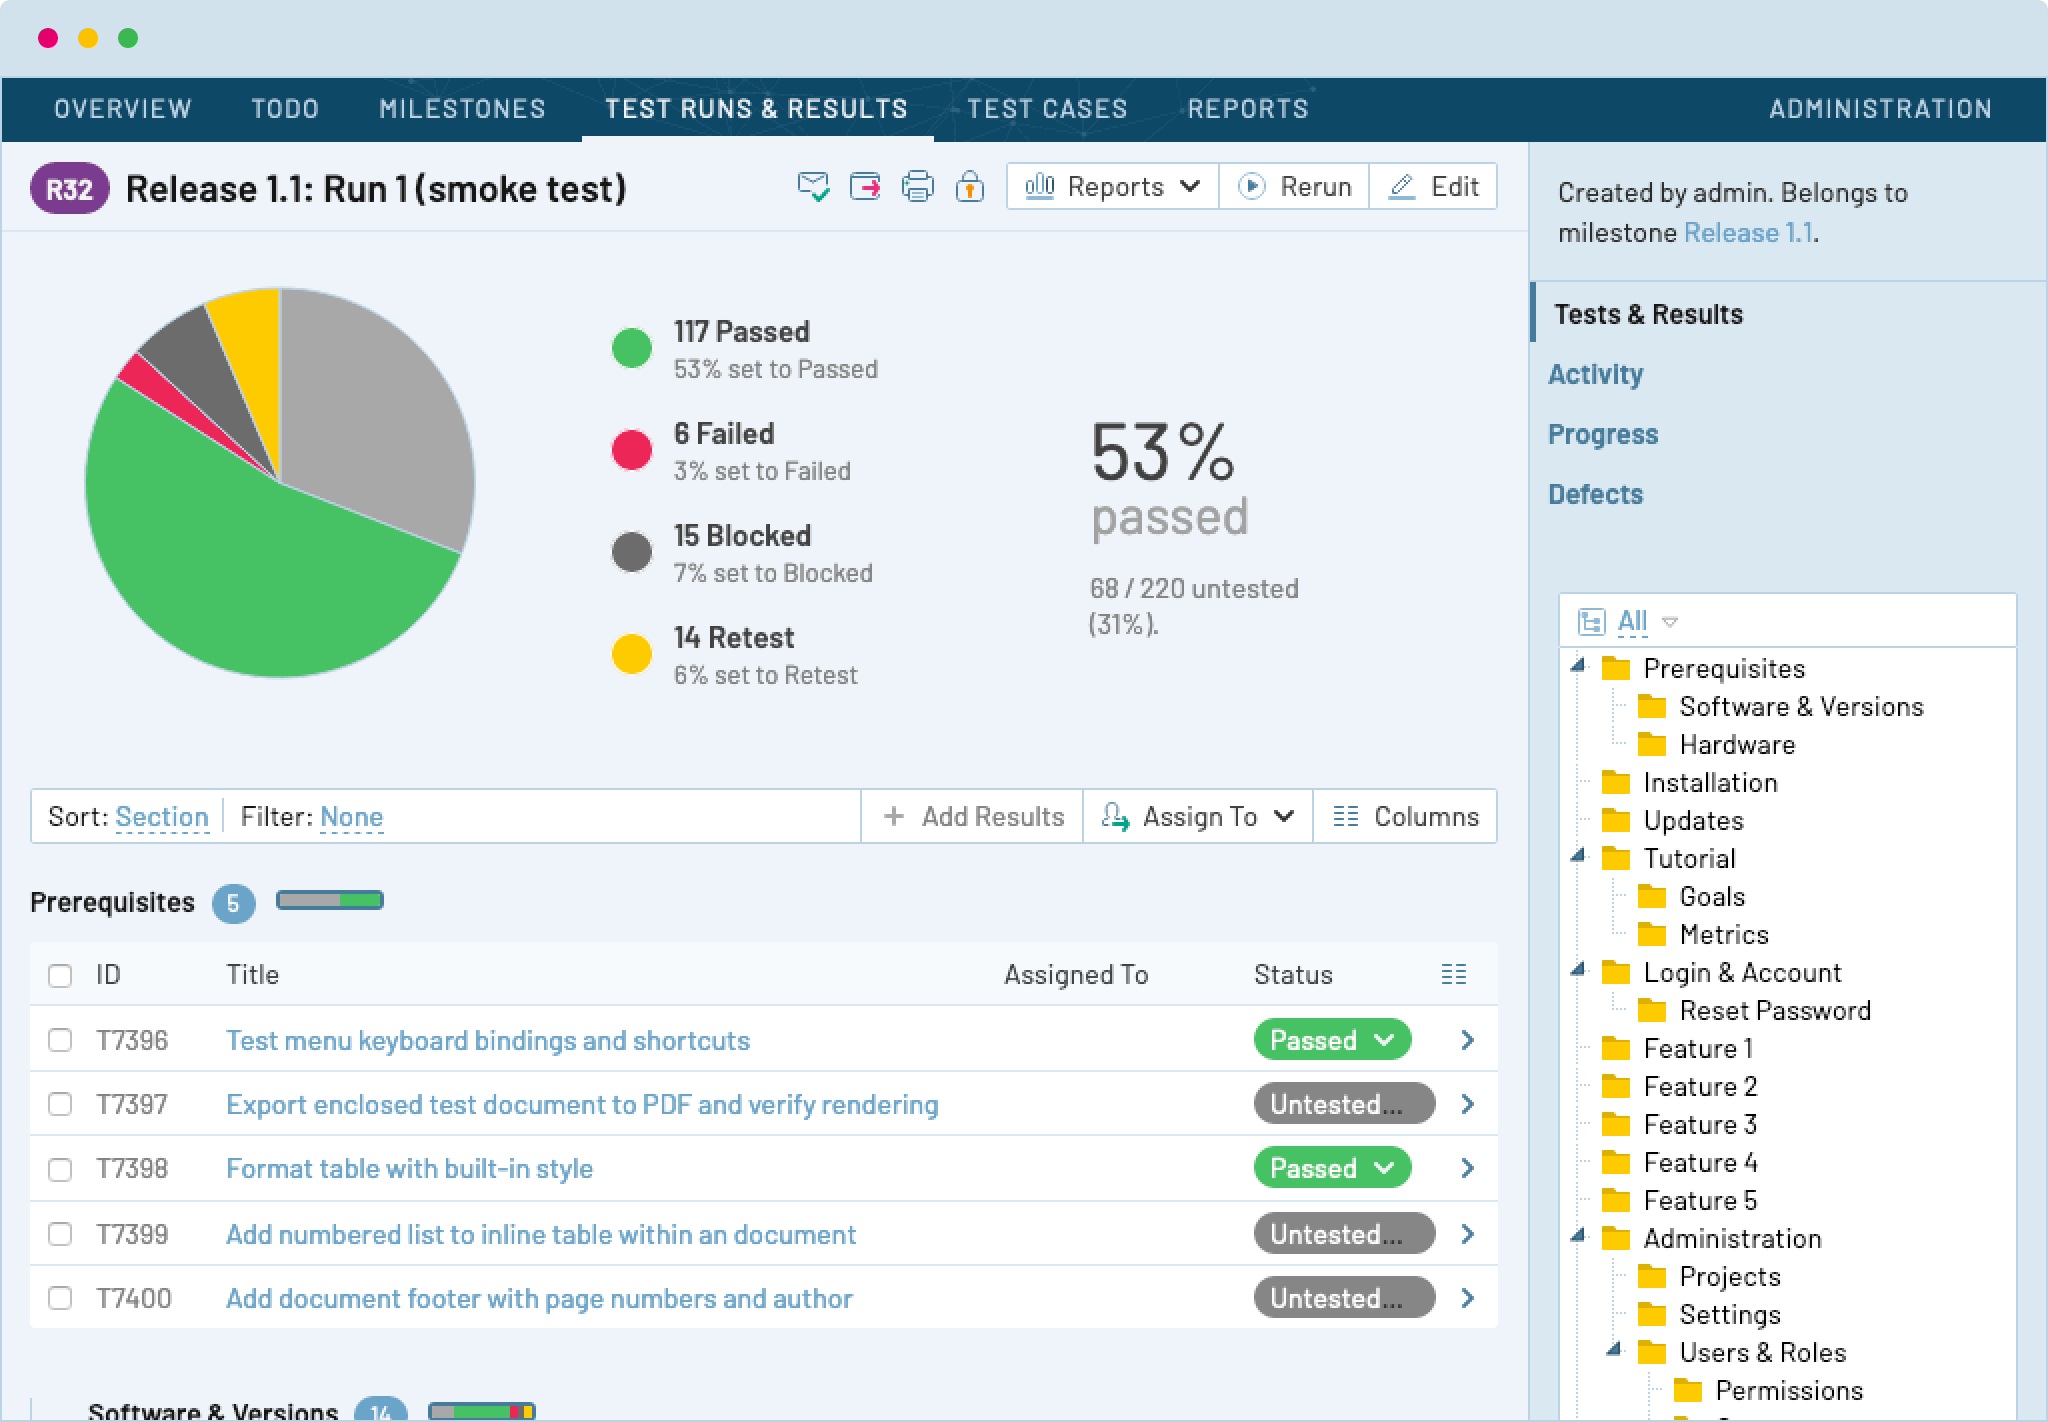
\includegraphics[width=6.5cm]{./imagenes/testrail.png} 
	\end{center}
    \item TESTPAD\\
Testpad utiliza planes de prueba inspirados en listas de verificación para pruebas ágiles, pruebas exploratorias, gestión de casos de prueba tradicional, BDD resaltado por sintaxis y mucho más. Es una herramienta liviana con un editor controlado por teclado y tiene una interfaz de usuario altamente receptiva impulsada por JavaScript.
\begin{center}
	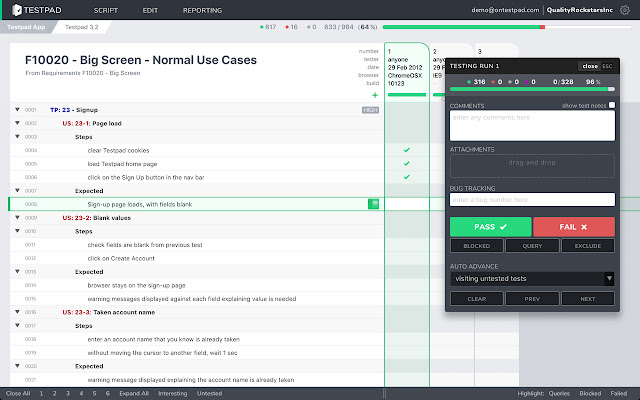
\includegraphics[width=6.5cm]{./imagenes/testpad.jpg} 
	\end{center}
    \item AWS CodePipeline\\
Servicio de entrega continua para actualizaciones de aplicaciones rápidas y confiables . CodePipeline compila, prueba e implementa su código cada vez que hay un cambio de código, según los modelos de proceso de lanzamiento que defina. ofrece modelado de flujo de trabajo, integraciones de AWS y complementos prediseñados.\\
\begin{center}
	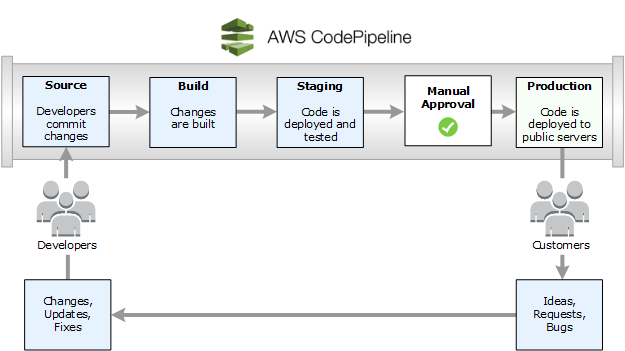
\includegraphics[width=6.5cm]{./imagenes/pipeline.png} 
	\end{center}
    \item Google Cloud Build\\
 Cloud Build permite crear software rápidamente.  control completo sobre la definición de flujos de trabajo personalizados para compilar, probar e implementar en múltiples entornos, como VM, sin servidor, Kubernetes o Firebase.
 \begin{center}
	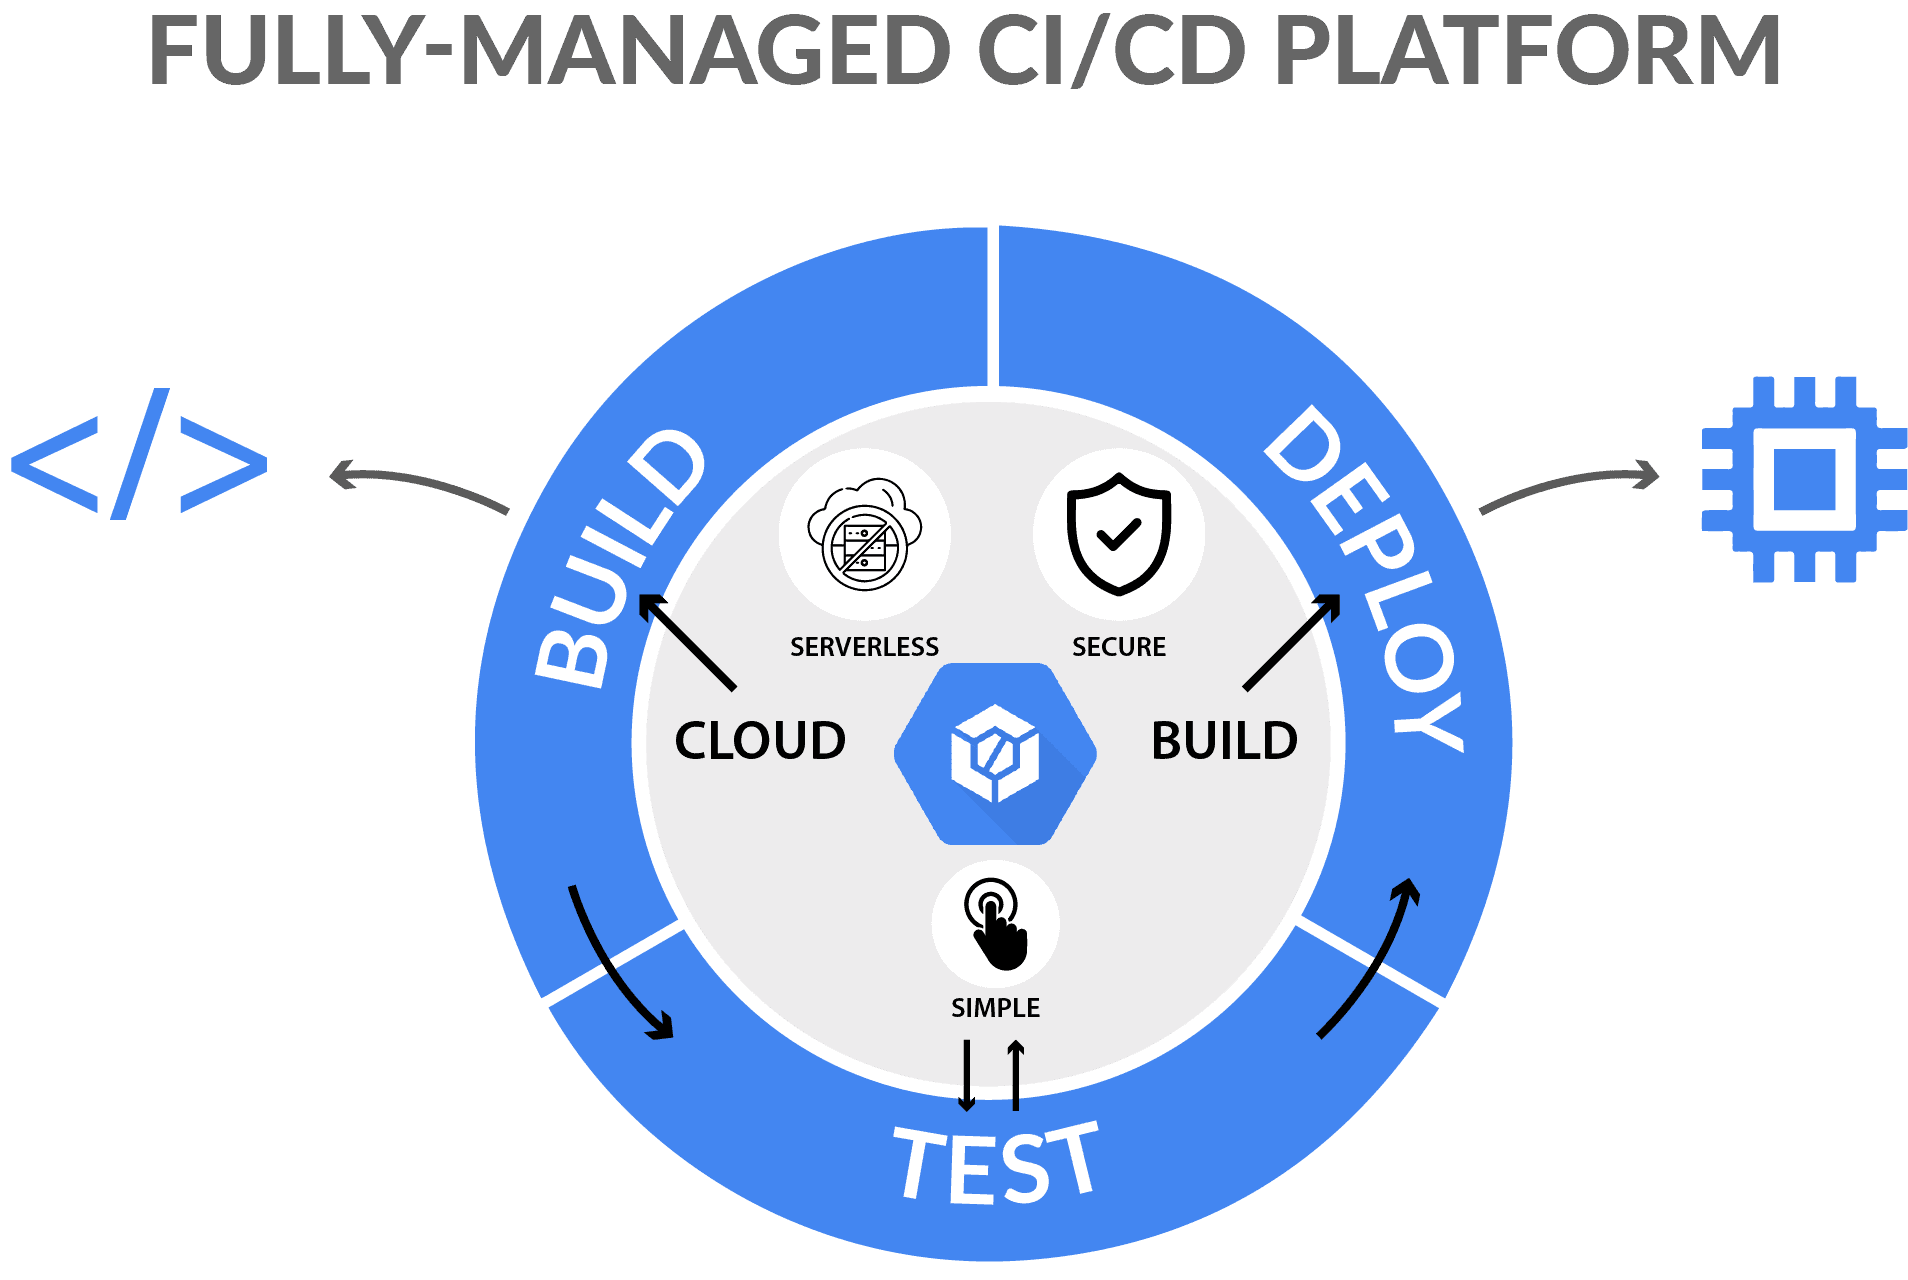
\includegraphics[width=6.5cm]{./imagenes/gcb.png} 
	\end{center}
 \item Github Actions\\
 GitHub Actions es una herramienta que permite reducir la cadena de acciones necesaria para la ejecución de código, mediante la creación de un de flujo de trabajo encargado del Pipeline. Siendo configurable para que GitHub reaccione a ciertos eventos de forma automática según nuestras preferencias.\\
 \begin{center}
	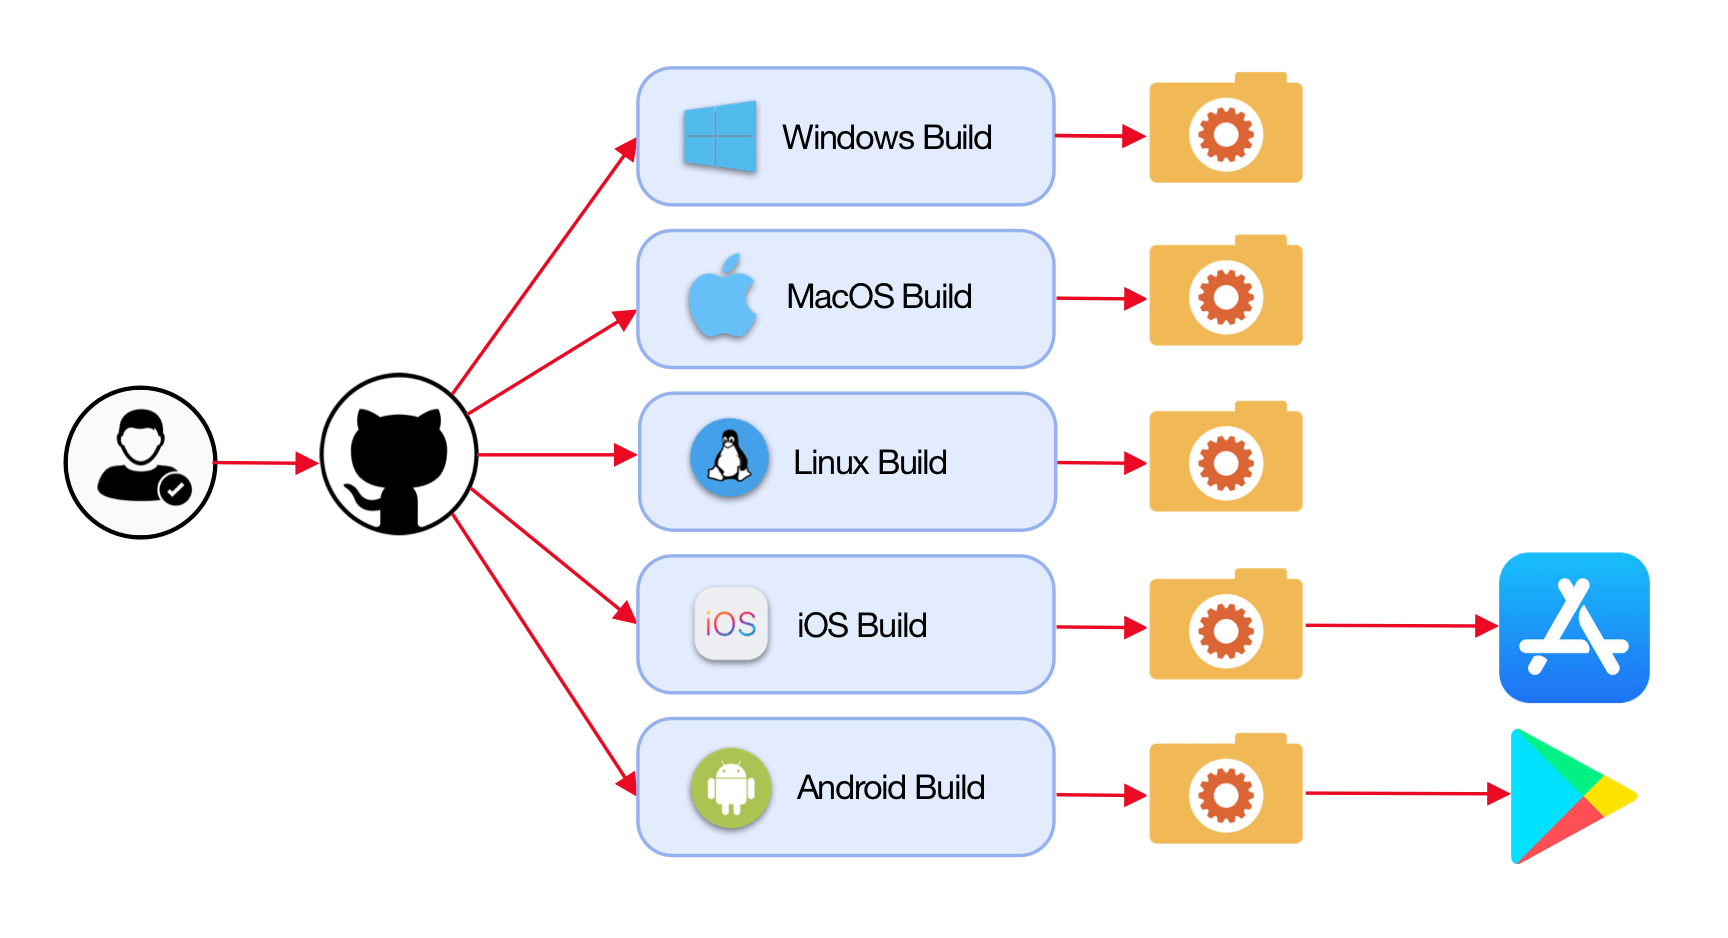
\includegraphics[width=7cm]{./imagenes/github.png} 
	\end{center}\\\\\\
 \item Azure DevOps\\
 Azure DevOps proporciona alojamiento Git privado ilimitado, compilación en la nube para la integración continua, planificación ágil y administración de versiones para la entrega continua en la nube y en las instalaciones. Incluye amplio soporte IDE.
Azure DevOps es una herramienta en la categoría de herramientas de entorno de desarrollo integrado de una pila tecnológica. Usado por empresas como Microsoft, QRPoint,BigClarity iOLAP.\\
\\Caracteristicas:\\
- Herramientas ágiles: tableros kanban, trabajos pendientes, tableros scrum
Informes: paneles, widgets, Power BI\\
- Git: repositorios privados gratuitos, solicitudes de extracción\\
- Integración continua: construcciones y diagnósticos automatizados\\
- Agentes de compilación en la nube: agentes multiplataforma para Windows, Mac y Linux\\
- Herramientas de prueba: pruebas unitarias, pruebas de carga, pruebas manuales, exploratorias y de aceptación del usuario\\
- Gestión de versiones: automatice implementaciones, flujos de trabajo de aprobación cerrados, pistas de auditoría\\
- Administración de paquetes: paquetes npm y NuGet de host\\
- Integración: enlace de código y versiones a elementos de trabajo, compilaciones y resultados de pruebas.

 \begin{center}
	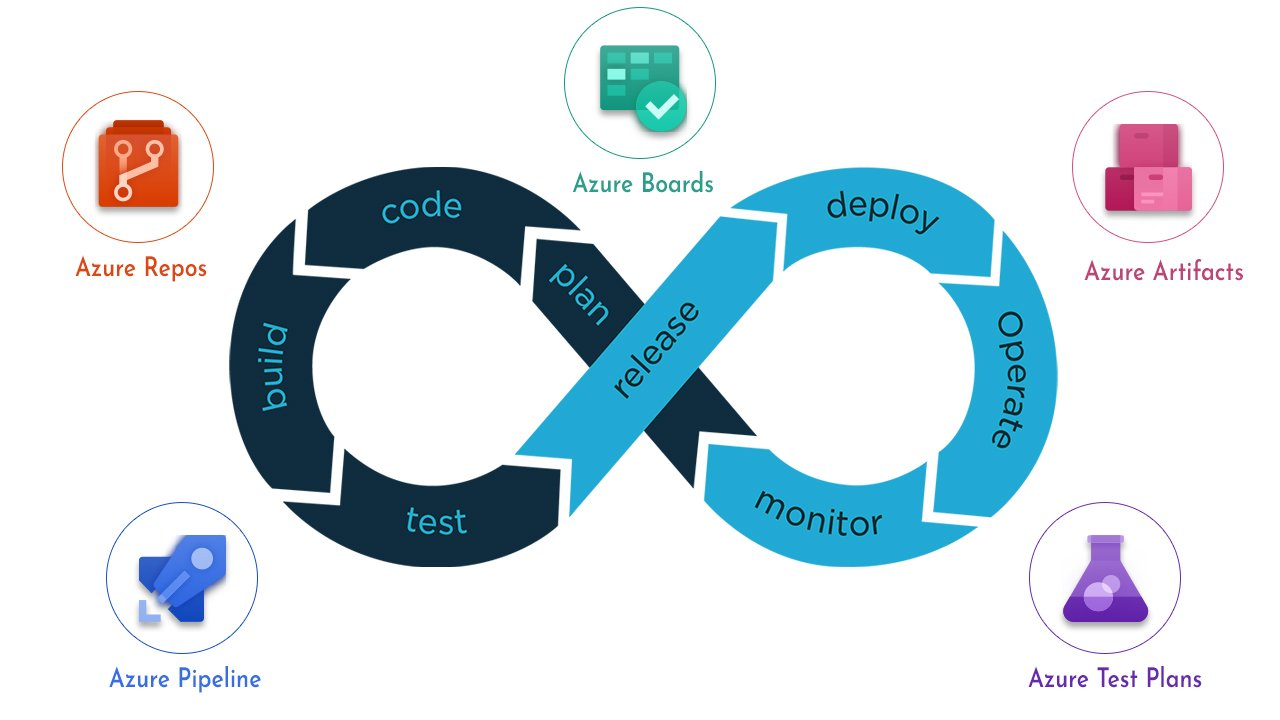
\includegraphics[width=6.5cm]{./imagenes/devops.jpeg} 
	\end{center}	
\end{itemize}
\section{Comparativa}
 \begin{center}
	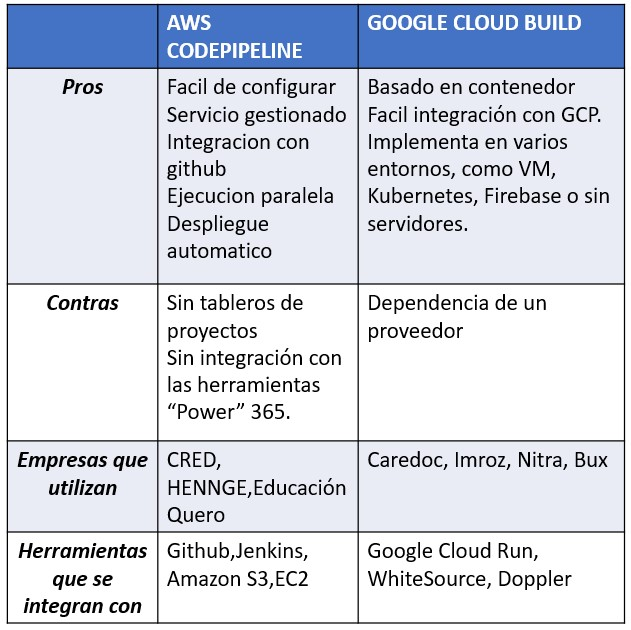
\includegraphics[width=7.5cm]{./imagenes/comparativa.jpg} 
	\end{center}

\section{Conclusiones}
Las pipelines han convertido en dos de los grandes proveedores de cloud pública y ofrecen tantísimos servicios que podemos encontrar sin dificultad soluciones que se adapten a nuestras necesidades, sean cuáles sea. nos permiten disponer en la nube de bases de datos, redes, herramientas de desarrollo y gestión, analytics, machine learning y mucho más. CodePipeline es otra característica revolucionaria de AWS que simplifica la forma de administrar su conjunto de herramientas CI / CD. Se integra con herramientas como GitHub, Jenkins y CodeDeploy que le permiten controlar visualmente el flujo de actualizaciones de aplicaciones desde la compilación hasta la producción. Se divide todo el ciclo de vida de la aplicación en una serie de etapas con cada etapa que consiste en una acción que se iniciará en su código. Al empujar una compilación al repositorio de Git, CodePipeline inicia la secuencia de acciones y pasa su código a cada etapa consecutiva automáticamente.
\section{Recomendaciones}
Utilice el cifrado y la autenticación para los repositorios de origen que se conectan a sus canalizaciones.
Utilice las prácticas recomendadas que se proporcionan en esta sección para las canalizaciones con un proveedor de acciones de Jenkins.
Puede crear canalizaciones que se integran con otrasAWSServicios de . Puede serAWSServicios de, como Amazon S3 o productos de terceros, como, por ejemplo, GitHub.


%----------------------------------------------------------------------------------------
%	REFERENCE LIST
%----------------------------------------------------------------------------------------
\newpage
\begin{thebibliography}{99}
\bibitem - Practicas recomendadas (2021) https://docs.aws.amazon.com/es_es/codepipeline/latest/userguide/best-practices.html/
	
	\bibitem - Alvarado Abarca, Miguel(2017)Metodología de implementación de aplicaciones de software  https://repositorio.una.ac.cr/handle/11056/14176
	\bibitem - Sierra Martin,Miguel (2021)Prácticas DevOps para la automatización de la integración https://oa.upm.es/68239/
    \bibitem - Mercado-Ramos, V. H., Zapata, J., & Ceballos, Y. F. (2015). Herramientas y buenas prácticas para el aseguramiento de calidad de software con metodologías ágiles. Revista de Investigación, Desarrollo e Innovación https://revistas.uptc.edu.co/index.php/investigacion_duitama/article/view/3277
    
    \bibitem - Escobar-Rivera, Dalilis; Moreno-Pino, Mayra Rosario; Cuevas-Rodríguez, Luis (2016).La calidad de la auditoría en Sistemas de Gestión. Software http://efaidnbmnnnibpcajpcglclefindmkaj/viewer.html?pdfurl=https%3A%2F%2Fwww.redalyc.org%2Fpdf%2F1815%2F181545579007.pdf&clen=1113189
    \bibitem - Tayché Capote-García (2015), Perspectivas del cuadro de mando integral personalizadas para laboratorios de pruebas de software. https://rii.cujae.edu.cu/index.php/revistaind/article/view/697
    \bibitem - Mera Paz, Julián Andrés (2016) , Análisis del proceso de pruebas de calidad de software.https://repository.ucc.edu.co/handle/20.500.12494/962
    \bibitem - Herramientas para la gestión de calidad de software (2015)http://www.pmoinformatica.com/2015/04/herramientas-gestion-calidad-software.html

	\end{thebibliography}

%----------------------------------------------------------------------------------------

\end{document}
